\documentclass{article}
\usepackage{orcidlink}
\usepackage{ragged2e}
\usepackage{graphicx}
\usepackage{caption}
\usepackage{subcaption}
\usepackage{hyperref}
\usepackage[autocite=superscript, style=nature]{biblatex}
\addbibresource{Manuscript.bib}
\graphicspath{ {./Figures/} }

\hypersetup{
  colorlinks   = true,
  urlcolor     = black,
  linkcolor    = black,
  citecolor   = black
}

\renewcommand{\thetable}{S\arabic{table}}
\renewcommand{\thefigure}{S\arabic{figure}}

\begin{document}

\section*{Supplementary Information}

\subsection*{Pilot run taxa}
Initial pilot runs were done on Bombus, Cetoniidae, Coccinellidae, Coleoptera, Lepidoptera, Odonata, Rodentia, and Zygaenidae. These taxa were chosen in order to test the machine learning pipeline on taxa with different levels of difficulty of identification. Rodentia were added to include a taxon outside of the Insecta.

\subsection*{Image recognition model configuration}
\label{sec:model}
Models were trained in Python 3.9\autocite{python}, using TensorFlow\autocite{tensorflow} and Keras\autocite{keras} to train a new recognition model based on the Inception-ResNet-v2 architecture\autocite{szegedy2016inceptionv4} for every dataset. A dense classification layer using softmax activation replaced the top layer of the Inception-ResNet-v2 model as a new top layer, with 17 nodes to classify each of the 17 species. For the loss function we used standard categorical cross entropy loss.

Color channels of input images were normalized between -1 and 1, and were scaled to 256\(\times\)256 pixels, cropping the image to become square if needed. Training data were augmented by shearing up to a factor of 0.2, zooming up to a factor of 0.2, rotating up to 90 degrees, and randomly flipping horizontally or not. Validation and test images were only normalized and squared, not augmented.

In the first training stage, the weights of the original Inception-ResNet-v2 layers were frozen, training only the newly added top layer. This was done for 2 epochs with a learning rate of \(1\cdot10^{-3}\). This has an equivalent effect as learning rate warm-up.

In the second training stage, all layers were trained. This was done for a maximum of 200 epochs, with an initial learning rate of \(1\cdot10^{-4}\). The learning rate was multiplied by 0.1 when the validation loss did not improve for 3 consecutive epochs. The minimum of the learning rate was set to \(1\cdot10^{-8}\).

After each epoch, model performance was evaluated using the validation set, saving the weights of the current model to disk as the latest checkpoint if the accuracy for the validation set had improved since the last saved checkpoint. Finally, when the model did not reduce its loss for 8 consecutive epochs, training was stopped. The most recently stored checkpoint was then used as the final recognition model for that dataset, and its performance measured using the test data.


\pagebreak
\subsection*{Taxonomic order result metrics}


\begin{table}[h!]
  \centering

  \begin{tabular}{|r | r | r|}
   \hline
   \textbf{Order} & \textbf{Bias in cs data with img} & \textbf{VoI (F\boldmath$_1$ increase \boldmath$\cdot10^{6}$)} \\ [0.5ex]
   \hline
   Asparagales & 5259 & 13.05 \\
   Lamiales & 3879 & 9.36 \\
   Polyporales & -11060 & 4.11 \\
   Lecanorales & -106853 & 1.72 \\
   Agaricales & -22932 & 1.52 \\
   Diptera & -110248 & 1.42 \\
   Coleoptera & -51782 & 1.09 \\
   Passeriformes & 28630 & 0.73 \\
   Odonata & 13075 & 0.32 \\
   Lepidoptera & 145110 & 0.17 \\
   Charadriiformes & 57421 & 0.13 \\
   Anseriformes & 49501 & 0.02 \\  [1ex]
   \hline
  \end{tabular}
  \caption{\footnotesize Orders used in the machine learning experiment, their over- or under-representation among citizen science observations with images (relative to all orders having an equal average amount of such observations per species), and the Value of Information as measured by the expected F\(_1\) increase for adding one observation with images to the number of observations with images currently available. Sorted by VoI (descending). These are the numerical values for figure \ref{fig:VoI_vs_bias}.}
  \label{tab:biases}
  \end{table}

  \pagebreak
  \subsection*{Von Bertalanffy Growth Curves}

 
  \begin{figure}[!ht]
    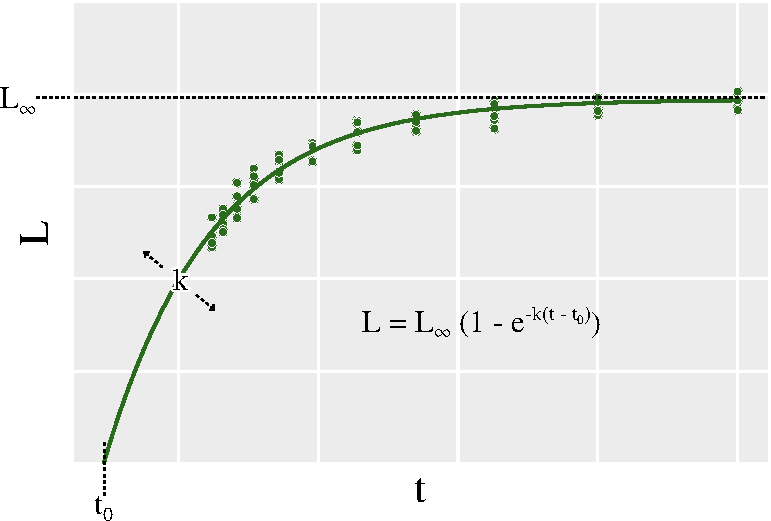
\includegraphics[width=\textwidth]{6}
    \caption{\footnotesize Visualization of the Von Bertalanffy Growth Curve parameters. Curves were fitted using the Levenberg-Marquardt (Least Squares) algorithm. Residuals were plotted for each taxon and not found to be heterogeneous in their distribution.}
    \label{fig:vbgf}
  \end{figure} 
  \printbibliography

\end{document}
